% Options for packages loaded elsewhere
\PassOptionsToPackage{unicode}{hyperref}
\PassOptionsToPackage{hyphens}{url}
%
\documentclass[
]{article}
\usepackage{amsmath,amssymb}
\usepackage{lmodern}
\usepackage{ifxetex,ifluatex}
\ifnum 0\ifxetex 1\fi\ifluatex 1\fi=0 % if pdftex
  \usepackage[T1]{fontenc}
  \usepackage[utf8]{inputenc}
  \usepackage{textcomp} % provide euro and other symbols
\else % if luatex or xetex
  \usepackage{unicode-math}
  \defaultfontfeatures{Scale=MatchLowercase}
  \defaultfontfeatures[\rmfamily]{Ligatures=TeX,Scale=1}
\fi
% Use upquote if available, for straight quotes in verbatim environments
\IfFileExists{upquote.sty}{\usepackage{upquote}}{}
\IfFileExists{microtype.sty}{% use microtype if available
  \usepackage[]{microtype}
  \UseMicrotypeSet[protrusion]{basicmath} % disable protrusion for tt fonts
}{}
\makeatletter
\@ifundefined{KOMAClassName}{% if non-KOMA class
  \IfFileExists{parskip.sty}{%
    \usepackage{parskip}
  }{% else
    \setlength{\parindent}{0pt}
    \setlength{\parskip}{6pt plus 2pt minus 1pt}}
}{% if KOMA class
  \KOMAoptions{parskip=half}}
\makeatother
\usepackage{xcolor}
\IfFileExists{xurl.sty}{\usepackage{xurl}}{} % add URL line breaks if available
\IfFileExists{bookmark.sty}{\usepackage{bookmark}}{\usepackage{hyperref}}
\hypersetup{
  pdftitle={scRNA},
  pdfauthor={Maria Lucia Romero},
  hidelinks,
  pdfcreator={LaTeX via pandoc}}
\urlstyle{same} % disable monospaced font for URLs
\usepackage[margin=1in]{geometry}
\usepackage{color}
\usepackage{fancyvrb}
\newcommand{\VerbBar}{|}
\newcommand{\VERB}{\Verb[commandchars=\\\{\}]}
\DefineVerbatimEnvironment{Highlighting}{Verbatim}{commandchars=\\\{\}}
% Add ',fontsize=\small' for more characters per line
\usepackage{framed}
\definecolor{shadecolor}{RGB}{248,248,248}
\newenvironment{Shaded}{\begin{snugshade}}{\end{snugshade}}
\newcommand{\AlertTok}[1]{\textcolor[rgb]{0.94,0.16,0.16}{#1}}
\newcommand{\AnnotationTok}[1]{\textcolor[rgb]{0.56,0.35,0.01}{\textbf{\textit{#1}}}}
\newcommand{\AttributeTok}[1]{\textcolor[rgb]{0.77,0.63,0.00}{#1}}
\newcommand{\BaseNTok}[1]{\textcolor[rgb]{0.00,0.00,0.81}{#1}}
\newcommand{\BuiltInTok}[1]{#1}
\newcommand{\CharTok}[1]{\textcolor[rgb]{0.31,0.60,0.02}{#1}}
\newcommand{\CommentTok}[1]{\textcolor[rgb]{0.56,0.35,0.01}{\textit{#1}}}
\newcommand{\CommentVarTok}[1]{\textcolor[rgb]{0.56,0.35,0.01}{\textbf{\textit{#1}}}}
\newcommand{\ConstantTok}[1]{\textcolor[rgb]{0.00,0.00,0.00}{#1}}
\newcommand{\ControlFlowTok}[1]{\textcolor[rgb]{0.13,0.29,0.53}{\textbf{#1}}}
\newcommand{\DataTypeTok}[1]{\textcolor[rgb]{0.13,0.29,0.53}{#1}}
\newcommand{\DecValTok}[1]{\textcolor[rgb]{0.00,0.00,0.81}{#1}}
\newcommand{\DocumentationTok}[1]{\textcolor[rgb]{0.56,0.35,0.01}{\textbf{\textit{#1}}}}
\newcommand{\ErrorTok}[1]{\textcolor[rgb]{0.64,0.00,0.00}{\textbf{#1}}}
\newcommand{\ExtensionTok}[1]{#1}
\newcommand{\FloatTok}[1]{\textcolor[rgb]{0.00,0.00,0.81}{#1}}
\newcommand{\FunctionTok}[1]{\textcolor[rgb]{0.00,0.00,0.00}{#1}}
\newcommand{\ImportTok}[1]{#1}
\newcommand{\InformationTok}[1]{\textcolor[rgb]{0.56,0.35,0.01}{\textbf{\textit{#1}}}}
\newcommand{\KeywordTok}[1]{\textcolor[rgb]{0.13,0.29,0.53}{\textbf{#1}}}
\newcommand{\NormalTok}[1]{#1}
\newcommand{\OperatorTok}[1]{\textcolor[rgb]{0.81,0.36,0.00}{\textbf{#1}}}
\newcommand{\OtherTok}[1]{\textcolor[rgb]{0.56,0.35,0.01}{#1}}
\newcommand{\PreprocessorTok}[1]{\textcolor[rgb]{0.56,0.35,0.01}{\textit{#1}}}
\newcommand{\RegionMarkerTok}[1]{#1}
\newcommand{\SpecialCharTok}[1]{\textcolor[rgb]{0.00,0.00,0.00}{#1}}
\newcommand{\SpecialStringTok}[1]{\textcolor[rgb]{0.31,0.60,0.02}{#1}}
\newcommand{\StringTok}[1]{\textcolor[rgb]{0.31,0.60,0.02}{#1}}
\newcommand{\VariableTok}[1]{\textcolor[rgb]{0.00,0.00,0.00}{#1}}
\newcommand{\VerbatimStringTok}[1]{\textcolor[rgb]{0.31,0.60,0.02}{#1}}
\newcommand{\WarningTok}[1]{\textcolor[rgb]{0.56,0.35,0.01}{\textbf{\textit{#1}}}}
\usepackage{graphicx}
\makeatletter
\def\maxwidth{\ifdim\Gin@nat@width>\linewidth\linewidth\else\Gin@nat@width\fi}
\def\maxheight{\ifdim\Gin@nat@height>\textheight\textheight\else\Gin@nat@height\fi}
\makeatother
% Scale images if necessary, so that they will not overflow the page
% margins by default, and it is still possible to overwrite the defaults
% using explicit options in \includegraphics[width, height, ...]{}
\setkeys{Gin}{width=\maxwidth,height=\maxheight,keepaspectratio}
% Set default figure placement to htbp
\makeatletter
\def\fps@figure{htbp}
\makeatother
\setlength{\emergencystretch}{3em} % prevent overfull lines
\providecommand{\tightlist}{%
  \setlength{\itemsep}{0pt}\setlength{\parskip}{0pt}}
\setcounter{secnumdepth}{-\maxdimen} % remove section numbering
\usepackage{booktabs}
\usepackage{longtable}
\usepackage{array}
\usepackage{multirow}
\usepackage{wrapfig}
\usepackage{float}
\usepackage{colortbl}
\usepackage{pdflscape}
\usepackage{tabu}
\usepackage{threeparttable}
\usepackage{threeparttablex}
\usepackage[normalem]{ulem}
\usepackage{makecell}
\usepackage{xcolor}
\ifluatex
  \usepackage{selnolig}  % disable illegal ligatures
\fi

\title{scRNA}
\author{Maria Lucia Romero}
\date{11/25/2021}

\begin{document}
\maketitle

\begin{Shaded}
\begin{Highlighting}[]
\FunctionTok{library}\NormalTok{(dplyr)}
\FunctionTok{library}\NormalTok{(reshape2)}
\FunctionTok{library}\NormalTok{(kableExtra)}
\FunctionTok{library}\NormalTok{(ggplot2)}
\FunctionTok{library}\NormalTok{(ggpubr)}
\FunctionTok{library}\NormalTok{(ggrepel)}
\FunctionTok{library}\NormalTok{(corrplot)}
\FunctionTok{library}\NormalTok{(RColorBrewer)}
\FunctionTok{library}\NormalTok{(plyr)}
\end{Highlighting}
\end{Shaded}

\hypertarget{loading-data}{%
\section{Loading data}\label{loading-data}}

\begin{Shaded}
\begin{Highlighting}[]
\NormalTok{RNAseq.data.mapping}\OtherTok{\textless{}{-}}\FunctionTok{read.csv}\NormalTok{(}\StringTok{"/Users/mlromeror/Documents/Sample co7dzuup\_xuczw9vc/data/data/cellranger\_mapping\_metrics\_hashed.csv"}\NormalTok{)}
\NormalTok{Multiome.RNAseq.data.mapping}\OtherTok{\textless{}{-}}\FunctionTok{read.csv}\NormalTok{(}\StringTok{"/Users/mlromeror/Documents/Sample co7dzuup\_xuczw9vc/data/data/cellranger\_mapping\_metrics\_multiome.csv"}\NormalTok{)}

\CommentTok{\#metadata\_multiome\textless{}{-} read.csv("/Users/mlromeror/Documents/Sample co7dzuup\_xuczw9vc/data/data/tonsil\_atlas\_metadata\_multiome.csv")}
\end{Highlighting}
\end{Shaded}

\begin{Shaded}
\begin{Highlighting}[]
\CommentTok{\#add a column }
\NormalTok{RNAseq.data.mapping}\SpecialCharTok{$}\NormalTok{method}\OtherTok{\textless{}{-}}\StringTok{"scRNAseq"}
\NormalTok{Multiome.RNAseq.data.mapping}\SpecialCharTok{$}\NormalTok{method}\OtherTok{\textless{}{-}}\StringTok{"multiome"}
\end{Highlighting}
\end{Shaded}

\hypertarget{mapping-data-table}{%
\section{Mapping data Table}\label{mapping-data-table}}

\begin{table}

\caption{\label{tab:unnamed-chunk-6}Visualization of mapping data}
\centering
\begin{tabular}[t]{l|l|l|l|l|l|l|l|l|l|l|l|l|l|l|l|l|l|l|l|l|l|l|l|l|l|l|l|l|l|l|l|l|l|l|l}
\hline
  & gem\_id & Estimated.Number.of.Cells & Mean.Reads.per.Cell & Median.Genes.per.Cell & Number.of.Reads & Valid.Barcodes & Sequencing.Saturation & Q30.Bases.in.Barcode & Q30.Bases.in.RNA.Read & Q30.Bases.in.UMI & Reads.Mapped.to.Genome & Reads.Mapped.Confidently.to.Genome & Reads.Mapped.Confidently.to.Intergenic.Regions & Reads.Mapped.Confidently.to.Intronic.Regions & Reads.Mapped.Confidently.to.Exonic.Regions & Reads.Mapped.Confidently.to.Transcriptome & Reads.Mapped.Antisense.to.Gene & Fraction.Reads.in.Cells & Total.Genes.Detected & Median.UMI.Counts.per.Cell & Antibody..Number.of.Reads & Antibody..Mean.Reads.per.Cell & Antibody..Valid.Barcodes & Antibody..Sequencing.Saturation & Antibody..Q30.Bases.in.Barcode & Antibody..Q30.Bases.in.Antibody.Read & Antibody..Q30.Bases.in.UMI & Antibody..Fraction.Antibody.Reads & Antibody..Fraction.Antibody.Reads.Usable & Antibody..Antibody.Reads.Usable.per.Cell & Antibody..Fraction.Reads.in.Barcodes.with.High.UMI.Counts & Antibody..Fraction.Unrecognized.Antibody & Antibody..Antibody.Reads.in.Cells & Antibody..Median.UMIs.per.Cell..summed.over.all.recognized.antibody.barcodes. & method\\
\hline
1 & izi9unx1\_8qdzhivu & 19,580 & 20,071 & 565 & 393,002,015 & 97.4\% & 62.4\% & 97.4\% & 91.6\% & 97.4\% & 96.9\% & 90.6\% & 5.5\% & 26.6\% & 58.5\% & 56.0\% & 1.3\% & 83.3\% & 25,933 & 1,576 & 8,720,503 & 445 & 98.8\% & 23.4\% & 99.5\% & 43.0\% & 99.4\% & 95.2\% & 48.3\% & 214 & 0.0\% & 4.8\% & 51.3\% & 90 & scRNAseq\\
\hline
2 & d8kwy76j\_7blj9otf & 23,458 & 21,100 & 1,176 & 494,981,784 & 97.1\% & 41.1\% & 96.9\% & 80.8\% & 96.7\% & 77.5\% & 74.2\% & 3.8\% & 28.3\% & 42.1\% & 38.9\% & 1.9\% & 90.6\% & 26,588 & 2,800 & 38,157,086 & 1,626 & 99.0\% & 33.3\% & 97.7\% & 65.1\% & 97.6\% & 96.5\% & 60.8\% & 989 & 0.0\% & 3.5\% & 63.7\% & 322 & scRNAseq\\
\hline
3 & giz3qso4\_783dbpu6 & 24,248 & 32,838 & 1,440 & 796,264,647 & 97.0\% & 52.1\% & 96.1\% & 80.7\% & 96.3\% & 79.4\% & 76.3\% & 3.4\% & 24.3\% & 48.7\% & 44.8\% & 1.8\% & 88.4\% & 27,319 & 3,975 & 59,277,922 & 2,444 & 99.0\% & 35.1\% & 97.7\% & 64.8\% & 97.6\% & 97.1\% & 63.4\% & 1,550 & 0.0\% & 2.9\% & 65.9\% & 473 & scRNAseq\\
\hline
4 & i5udk3x0\_57gv6ncx & 18,680 & 23,720 & 1,312 & 443,092,189 & 97.4\% & 41.8\% & 96.2\% & 80.3\% & 96.1\% & 78.3\% & 74.7\% & 3.6\% & 21.5\% & 49.6\% & 45.9\% & 1.6\% & 87.2\% & 26,161 & 3,474 & 29,588,501 & 1,583 & 98.9\% & 35.6\% & 97.8\% & 64.8\% & 97.6\% & 96.4\% & 47.2\% & 747 & 0.0\% & 3.6\% & 49.4\% & 244 & scRNAseq\\
\hline
5 & umt51kfr\_p8ei65ms & 21,126 & 30,271 & 1,476 & 639,514,672 & 97.4\% & 47.2\% & 96.2\% & 80.0\% & 96.1\% & 76.6\% & 73.2\% & 3.6\% & 22.4\% & 47.1\% & 43.7\% & 1.6\% & 89.8\% & 26,885 & 3,875 & 20,489,244 & 969 & 98.9\% & 33.7\% & 97.7\% & 65.5\% & 97.5\% & 96.8\% & 51.6\% & 500 & 0.0\% & 3.2\% & 53.9\% & 157 & scRNAseq\\
\hline
6 & bw94nf57\_vm85woki & 24,024 & 26,566 & 1,481 & 638,235,233 & 96.6\% & 48.6\% & 97.0\% & 94.5\% & 97.0\% & 96.7\% & 91.6\% & 4.5\% & 31.6\% & 55.5\% & 50.6\% & 3.3\% & 85.2\% & 27,026 & 3,920 & 22,830,949 & 950 & 98.8\% & 45.3\% & 97.8\% & 61.7\% & 97.4\% & 92.9\% & 51.8\% & 491 & 0.0\% & 7.1\% & 56.3\% & 203 & scRNAseq\\
\hline
7 & ggq3nifm\_jkilwp1x & 27,379 & 26,026 & 1,451 & 712,583,457 & 96.8\% & 49.0\% & 96.9\% & 95.0\% & 96.9\% & 97.1\% & 92.3\% & 4.4\% & 30.4\% & 57.5\% & 52.8\% & 3.1\% & 86.4\% & 27,247 & 3,949 & 22,947,172 & 838 & 98.9\% & 48.1\% & 97.8\% & 61.0\% & 97.4\% & 92.7\% & 52.0\% & 435 & 0.0\% & 7.3\% & 56.6\% & 177 & scRNAseq\\
\hline
8 & dvcbn9p8\_ix0j3k8b & 28,659 & 28,604 & 1,481 & 819,787,582 & 97.0\% & 52.3\% & 96.9\% & 95.0\% & 97.1\% & 97.5\% & 92.3\% & 4.4\% & 30.3\% & 57.7\% & 53.4\% & 2.8\% & 83.0\% & 27,755 & 3,954 & 25,757,716 & 898 & 99.0\% & 44.6\% & 98.4\% & 64.2\% & 98.5\% & 92.6\% & 50.9\% & 457 & 0.0\% & 7.4\% & 55.5\% & 101 & scRNAseq\\
\hline
9 & ff8s19u3\_7e96iusr & 30,163 & 30,092 & 1,595 & 907,683,518 & 97.1\% & 51.7\% & 97.5\% & 95.7\% & 97.7\% & 97.6\% & 93.4\% & 4.1\% & 29.3\% & 60.1\% & 56.2\% & 2.5\% & 84.2\% & 27,903 & 4,608 & 28,053,180 & 930 & 99.0\% & 40.5\% & 98.3\% & 64.3\% & 98.4\% & 93.3\% & 53.6\% & 498 & 0.0\% & 6.7\% & 58.1\% & 123 & scRNAseq\\
\hline
10 & dvdzq8et\_eot75su8 & 19,053 & 49,439 & 1,924 & 941,975,034 & 96.8\% & 65.2\% & 96.3\% & 93.9\% & 95.3\% & 97.4\% & 92.8\% & 4.3\% & 24.3\% & 64.1\% & 60.8\% & 1.9\% & 85.0\% & 27,080 & 5,888 & 157,876,755 & 8,286 & 98.8\% & 63.7\% & 97.7\% & 68.2\% & 97.7\% & 91.7\% & 46.3\% & 3,839 & 0.0\% & 8.3\% & 51.0\% & 560 & scRNAseq\\
\hline
11 & md651vbh\_eymr91s7 & 19,024 & 28,417 & 1,738 & 540,617,235 & 96.7\% & 41.9\% & 96.9\% & 93.1\% & 97.1\% & 96.1\% & 88.5\% & 5.6\% & 39.4\% & 43.4\% & 39.4\% & 2.9\% & 89.0\% & 27,364 & 4,652 & 259,411,291 & 13,636 & 98.8\% & 36.2\% & 97.1\% & 69.3\% & 97.1\% & 96.0\% & 56.4\% & 7,695 & 1.2\% & 4.0\% & 59.5\% & 3,241 & scRNAseq\\
\hline
12 & n1b3su0a\_l7shyi35 & 12,826 & 57,650 & 1,714 & 739,430,260 & 96.5\% & 68.3\% & 96.9\% & 93.1\% & 97.0\% & 95.9\% & 86.5\% & 6.7\% & 34.5\% & 45.4\% & 42.2\% & 2.1\% & 87.2\% & 26,700 & 4,754 & 179,391,632 & 13,986 & 98.9\% & 50.5\% & 97.0\% & 68.5\% & 97.1\% & 96.1\% & 44.0\% & 6,151 & 28.9\% & 3.9\% & 46.2\% & 2,036 & scRNAseq\\
\hline
13 & x739d5z1\_dsamhgey & 15,457 & 41,386 & 1,676 & 639,715,891 & 96.9\% & 63.5\% & 96.8\% & 92.5\% & 97.0\% & 97.3\% & 91.5\% & 4.7\% & 26.8\% & 60.1\% & 56.5\% & 2.1\% & 81.8\% & 26,501 & 4,746 & 186,717,642 & 12,079 & 98.8\% & 67.5\% & 97.8\% & 68.4\% & 97.7\% & 91.3\% & 38.6\% & 4,663 & 0.0\% & 8.7\% & 42.7\% & 637 & scRNAseq\\
\hline
14 & bz5rpwtv\_kg7w108r & 24,661 & 35,722 & 1,630 & 880,952,803 & 96.7\% & 58.6\% & 97.1\% & 95.1\% & 97.0\% & 96.9\% & 92.1\% & 4.1\% & 24.7\% & 63.2\% & 59.6\% & 2.3\% & 84.4\% & 27,130 & 4,716 & 30,839,209 & 1,250 & 98.9\% & 50.2\% & 97.8\% & 60.6\% & 97.6\% & 93.0\% & 48.6\% & 608 & 0.0\% & 7.0\% & 52.8\% & 155 & scRNAseq\\
\hline
15 & wf4su8ny\_h4yj8bv7 & 24,646 & 19,400 & 1,312 & 478,139,842 & 96.6\% & 45.3\% & 96.6\% & 94.5\% & 96.6\% & 97.5\% & 92.6\% & 4.1\% & 25.3\% & 63.1\% & 59.4\% & 2.4\% & 84.3\% & 26,431 & 3,399 & 34,461,302 & 1,398 & 98.9\% & 52.4\% & 97.8\% & 60.6\% & 97.6\% & 93.2\% & 45.5\% & 636 & 0.0\% & 6.8\% & 49.4\% & 160 & scRNAseq\\
\hline
16 & kjzv2rwx\_sfomyxok & 29,443 & 25,818 & 1,384 & 760,188,511 & 98.1\% & 55.1\% & 97.1\% & 94.5\% & 96.8\% & 97.0\% & 93.1\% & 5.2\% & 33.7\% & 54.1\% & 51.2\% & 1.8\% & 88.4\% & 26,877 & 3,929 & 62,416,515 & 2,119 & 99.4\% & 45.3\% & 97.5\% & 62.1\% & 97.0\% & 94.6\% & 63.2\% & 1,339 & 0.0\% & 5.4\% & 67.2\% & 261 & scRNAseq\\
\hline
17 & v8g80gtx\_ps9bamz7 & 29,401 & 26,568 & 1,449 & 781,131,740 & 97.3\% & 51.0\% & 97.1\% & 94.4\% & 96.7\% & 96.4\% & 92.0\% & 5.4\% & 32.0\% & 54.6\% & 51.6\% & 1.8\% & 87.9\% & 27,087 & 4,472 & 44,542,968 & 1,515 & 99.0\% & 57.4\% & 97.6\% & 61.4\% & 97.0\% & 91.7\% & 56.9\% & 861 & 0.0\% & 8.3\% & 62.6\% & 163 & scRNAseq\\
\hline
18 & ejto2bae\_y5mydeam & 22,847 & 37,972 & 1,690 & 867,549,060 & 97.9\% & 64.6\% & 97.4\% & 95.2\% & 97.0\% & 98.0\% & 94.2\% & 4.6\% & 24.7\% & 64.9\% & 61.9\% & 1.8\% & 88.5\% & 26,938 & 5,884 & 55,571,687 & 2,432 & 99.2\% & 49.3\% & 97.3\% & 61.8\% & 96.6\% & 95.2\% & 53.5\% & 1,301 & 3.5\% & 4.8\% & 56.6\% & 233 & scRNAseq\\
\hline
19 & z3of7uaq\_mzbhy4tt & 23,056 & 36,070 & 1,676 & 831,630,600 & 98.0\% & 62.3\% & 97.3\% & 95.1\% & 96.9\% & 98.0\% & 94.1\% & 4.6\% & 23.9\% & 65.6\% & 62.6\% & 1.7\% & 88.4\% & 26,962 & 5,909 & 61,026,456 & 2,646 & 99.3\% & 49.3\% & 97.4\% & 61.7\% & 96.7\% & 95.4\% & 56.9\% & 1,507 & 2.4\% & 4.6\% & 60.1\% & 247 & scRNAseq\\
\hline
\end{tabular}
\end{table}

\hypertarget{fraction-of-read-in-cell-rna-seq}{%
\subsection{Fraction of read in cell RNA
seq}\label{fraction-of-read-in-cell-rna-seq}}

Fraction of high quality fragments with a valid barcode that are
associated with cell-containing partitions. High quality fragments are
defined as read pairs with a valid barcode that map to the nuclear
genome with mapping quality \textgreater{} 30, are not chimeric and not
duplicate. We expect to have more than 40\% of fraction of high quality
fragments in cell

\begin{Shaded}
\begin{Highlighting}[]
\FunctionTok{par}\NormalTok{(}\AttributeTok{mar=}\FunctionTok{c}\NormalTok{(}\DecValTok{8}\NormalTok{,}\DecValTok{4}\NormalTok{,}\DecValTok{2}\NormalTok{,}\DecValTok{2}\NormalTok{),}\AttributeTok{mgp=}\FunctionTok{c}\NormalTok{(}\DecValTok{3}\NormalTok{, }\DecValTok{1}\NormalTok{, }\DecValTok{0}\NormalTok{))}

\NormalTok{p}\OtherTok{\textless{}{-}} \FunctionTok{ggbarplot}\NormalTok{(RNAseq.data.mapping, }
          \AttributeTok{x=}\StringTok{"gem\_id"}\NormalTok{,}
           \AttributeTok{y=}\StringTok{"Fraction.Reads.in.Cells"}\NormalTok{,}
          \AttributeTok{fill=}\StringTok{"steelblue"}\NormalTok{,}
          \AttributeTok{lab.col =} \StringTok{"black"}\NormalTok{, }
          \AttributeTok{lab.pos =} \StringTok{"out"}\NormalTok{,}
          \AttributeTok{lab.size =} \DecValTok{3}\NormalTok{,}
          \AttributeTok{ggtheme =} \FunctionTok{theme\_pubr}\NormalTok{(}\AttributeTok{x.text.angle =} \DecValTok{45}\NormalTok{),}
          \AttributeTok{label =} \ConstantTok{TRUE}\NormalTok{,}
          \AttributeTok{title =} \StringTok{"Fraction of read in cell RNA seq"}
\NormalTok{          )}
\NormalTok{p}\SpecialCharTok{+}\FunctionTok{font}\NormalTok{(}\StringTok{"title"}\NormalTok{, }\AttributeTok{size =} \DecValTok{12}\NormalTok{, }\AttributeTok{face =} \StringTok{"bold.italic"}\NormalTok{)}
\end{Highlighting}
\end{Shaded}

\includegraphics{RNAseq_multiomeRNA_files/figure-latex/unnamed-chunk-7-1.pdf}

\begin{Shaded}
\begin{Highlighting}[]
\FunctionTok{par}\NormalTok{(}\AttributeTok{mar=}\FunctionTok{c}\NormalTok{(}\DecValTok{8}\NormalTok{,}\DecValTok{4}\NormalTok{,}\DecValTok{2}\NormalTok{,}\DecValTok{2}\NormalTok{),}\AttributeTok{mgp=}\FunctionTok{c}\NormalTok{(}\DecValTok{3}\NormalTok{, }\DecValTok{1}\NormalTok{, }\DecValTok{0}\NormalTok{))}

\NormalTok{p}\OtherTok{\textless{}{-}} \FunctionTok{ggbarplot}\NormalTok{(Multiome.RNAseq.data.mapping, }
          \AttributeTok{x=}\StringTok{"Sample.ID"}\NormalTok{,}
          \AttributeTok{y=}\StringTok{"GEX.Fraction.of.transcriptomic.reads.in.cells"}\NormalTok{,}
          \AttributeTok{fill=}\StringTok{"steelblue"}\NormalTok{,}
          \AttributeTok{lab.col =} \StringTok{"black"}\NormalTok{, }
          \AttributeTok{lab.pos =} \StringTok{"out"}\NormalTok{,}
          \AttributeTok{lab.size =} \DecValTok{3}\NormalTok{,}
          \AttributeTok{ggtheme =} \FunctionTok{theme\_pubr}\NormalTok{(}\AttributeTok{x.text.angle =} \DecValTok{45}\NormalTok{),}
          \AttributeTok{label =} \ConstantTok{TRUE}\NormalTok{,}
          \AttributeTok{title =} \StringTok{"GEX Fraction transcriptomic Reads in Cells"}
\NormalTok{          )}
\NormalTok{p}\SpecialCharTok{+}\FunctionTok{font}\NormalTok{(}\StringTok{"title"}\NormalTok{, }\AttributeTok{size =} \DecValTok{12}\NormalTok{, }\AttributeTok{face =} \StringTok{"bold.italic"}\NormalTok{)}
\end{Highlighting}
\end{Shaded}

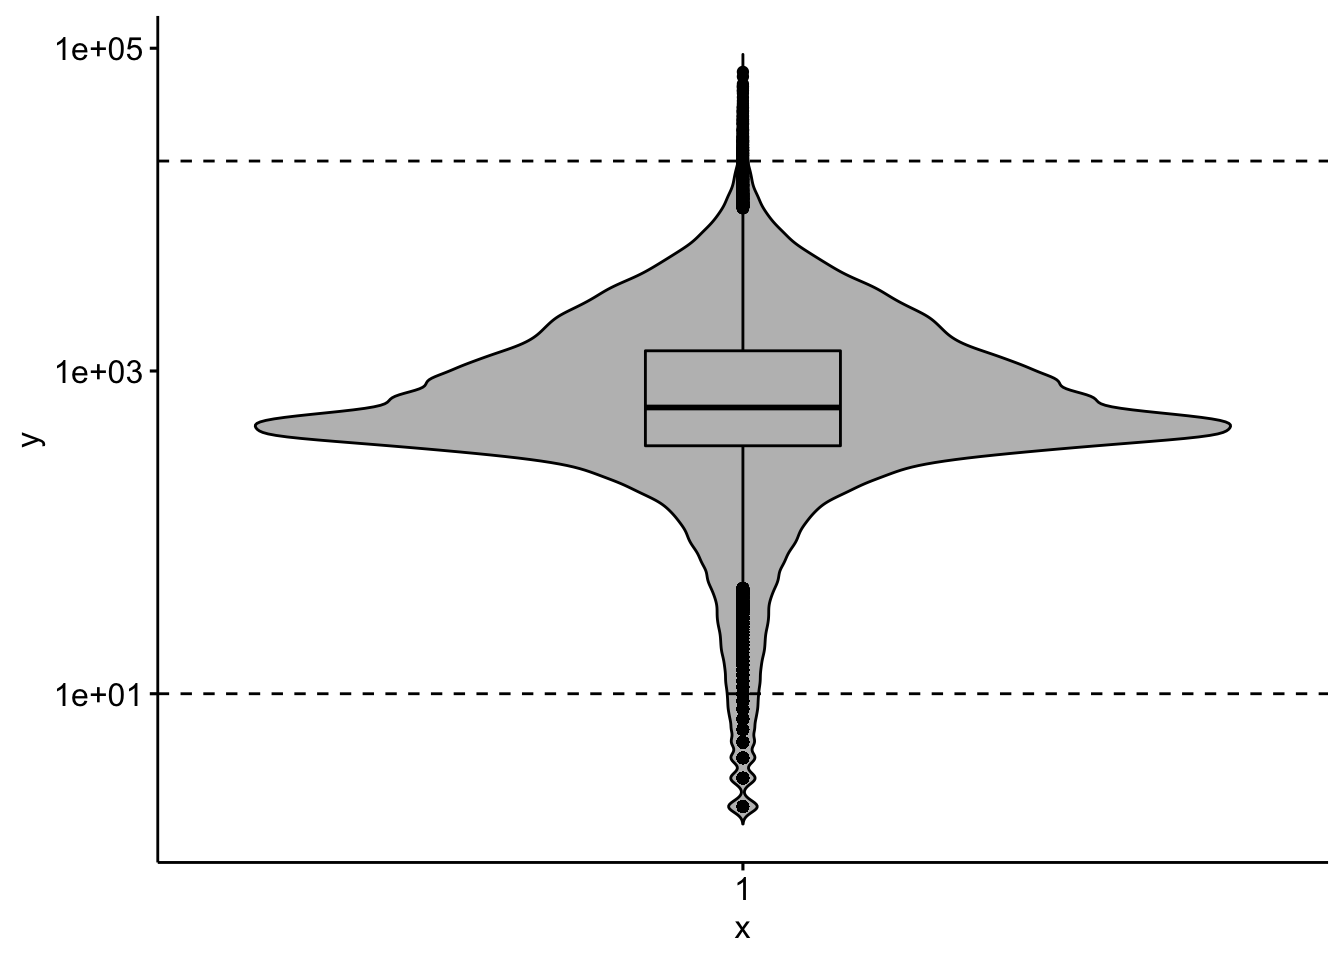
\includegraphics{RNAseq_multiomeRNA_files/figure-latex/unnamed-chunk-8-1.pdf}

\hypertarget{read-mapped-to-genome}{%
\subsection{Read Mapped to Genome}\label{read-mapped-to-genome}}

\hypertarget{rna-seq}{%
\subsubsection{RNA-seq}\label{rna-seq}}

\begin{Shaded}
\begin{Highlighting}[]
\FunctionTok{par}\NormalTok{(}\AttributeTok{mar=}\FunctionTok{c}\NormalTok{(}\DecValTok{8}\NormalTok{,}\DecValTok{4}\NormalTok{,}\DecValTok{2}\NormalTok{,}\DecValTok{2}\NormalTok{),}\AttributeTok{mgp=}\FunctionTok{c}\NormalTok{(}\DecValTok{3}\NormalTok{, }\DecValTok{1}\NormalTok{, }\DecValTok{0}\NormalTok{))}
\NormalTok{p}\OtherTok{\textless{}{-}} \FunctionTok{ggbarplot}\NormalTok{(RNAseq.data.mapping, }
          \AttributeTok{x=}\StringTok{"gem\_id"}\NormalTok{,}
           \AttributeTok{y=}\StringTok{"Reads.Mapped.to.Genome"}\NormalTok{,}
          \AttributeTok{fill=}\StringTok{"steelblue"}\NormalTok{,}
          \AttributeTok{lab.col =} \StringTok{"black"}\NormalTok{, }
          \AttributeTok{lab.pos =} \StringTok{"out"}\NormalTok{,}
          \AttributeTok{lab.size =} \DecValTok{3}\NormalTok{,}
          \AttributeTok{ggtheme =} \FunctionTok{theme\_pubr}\NormalTok{(}\AttributeTok{x.text.angle =} \DecValTok{45}\NormalTok{),}
          \AttributeTok{label =} \ConstantTok{TRUE}\NormalTok{,}
          \AttributeTok{title =} \StringTok{"Reads Mapped to Genome RNAseq"}
\NormalTok{          )}
\NormalTok{p}\SpecialCharTok{+}\FunctionTok{font}\NormalTok{(}\StringTok{"title"}\NormalTok{, }\AttributeTok{size =} \DecValTok{12}\NormalTok{, }\AttributeTok{face =} \StringTok{"bold.italic"}\NormalTok{)}
\end{Highlighting}
\end{Shaded}

\includegraphics{RNAseq_multiomeRNA_files/figure-latex/unnamed-chunk-9-1.pdf}

\hypertarget{gex-multiome}{%
\subsubsection{GEX multiome}\label{gex-multiome}}

\begin{Shaded}
\begin{Highlighting}[]
\NormalTok{p}\OtherTok{\textless{}{-}} \FunctionTok{ggbarplot}\NormalTok{(Multiome.RNAseq.data.mapping, }
          \AttributeTok{x=}\StringTok{"Sample.ID"}\NormalTok{,}
           \AttributeTok{y=}\StringTok{"GEX.Reads.mapped.to.genome"}\NormalTok{,}
          \AttributeTok{fill=}\StringTok{"steelblue"}\NormalTok{,}
          \AttributeTok{lab.col =} \StringTok{"black"}\NormalTok{, }
          \AttributeTok{lab.pos =} \StringTok{"out"}\NormalTok{,}
          \AttributeTok{lab.size =} \DecValTok{3}\NormalTok{,}
          \AttributeTok{ggtheme =} \FunctionTok{theme\_pubr}\NormalTok{(}\AttributeTok{x.text.angle =} \DecValTok{45}\NormalTok{),}
          \AttributeTok{label =} \ConstantTok{TRUE}\NormalTok{,}
          \AttributeTok{title =} \StringTok{"Reads Mapped to Genome GEX multiome"}
\NormalTok{          )}
\NormalTok{p}\SpecialCharTok{+}\FunctionTok{font}\NormalTok{(}\StringTok{"title"}\NormalTok{, }\AttributeTok{size =} \DecValTok{12}\NormalTok{, }\AttributeTok{face =} \StringTok{"bold.italic"}\NormalTok{)}
\end{Highlighting}
\end{Shaded}

\includegraphics{RNAseq_multiomeRNA_files/figure-latex/unnamed-chunk-10-1.pdf}

\hypertarget{compare-fraction-of-reads-mapped-between-rna-seq-and-multiome-gex}{%
\section{Compare Fraction of reads mapped between RNA-seq and Multiome
GEX}\label{compare-fraction-of-reads-mapped-between-rna-seq-and-multiome-gex}}

Now, we will compare the fraction of reads that are mapped to genome and
coffidently to genone and mapped to intergenic, intronic and exoni
regions between RNA-seq and Multiome methods.

\begin{Shaded}
\begin{Highlighting}[]
\NormalTok{RNAseq.data.fraction.melted}\OtherTok{\textless{}{-}}\FunctionTok{melt}\NormalTok{ (RNAseq.data.mapping[, }
                        \FunctionTok{c}\NormalTok{(}\StringTok{"gem\_id"}\NormalTok{, }
                                             \StringTok{"Reads.Mapped.to.Genome"}\NormalTok{,}
                                             \StringTok{"Reads.Mapped.Confidently.to.Genome"}\NormalTok{,}
                                             \StringTok{"Reads.Mapped.Confidently.to.Intergenic.Regions"}\NormalTok{,}
                                             \StringTok{"Reads.Mapped.Confidently.to.Intronic.Regions"}\NormalTok{,}
                                             \StringTok{"Reads.Mapped.Confidently.to.Exonic.Regions"}\NormalTok{)],}\AttributeTok{id.var=}\StringTok{"gem\_id"}\NormalTok{)}

\NormalTok{RNAseq.data.fraction.melted}\SpecialCharTok{$}\NormalTok{variable}\OtherTok{\textless{}{-}} \FunctionTok{revalue}\NormalTok{(RNAseq.data.fraction.melted}\SpecialCharTok{$}\NormalTok{variable,}
                                        \FunctionTok{c}\NormalTok{( }\StringTok{"Reads.Mapped.to.Genome"}\OtherTok{=}\StringTok{"Map.genome"}\NormalTok{, }
                                           \StringTok{"Reads.Mapped.Confidently.to.Genome"} \OtherTok{=} \StringTok{"Conf.map.genome"}\NormalTok{,}
                                           \StringTok{"Reads.Mapped.Confidently.to.Intergenic.Regions"}\OtherTok{=}\StringTok{"Intergenic"}\NormalTok{,}
                                           \StringTok{"Reads.Mapped.Confidently.to.Intronic.Regions"} \OtherTok{=} \StringTok{"Intronic"}\NormalTok{,}
        \StringTok{"Reads.Mapped.Confidently.to.Exonic.Regions"} \OtherTok{=} \StringTok{"Exonic"}\NormalTok{),}
        \AttributeTok{warn\_missing =} \ConstantTok{TRUE}\NormalTok{)}


\NormalTok{RNAseq.data.fraction.melted}\SpecialCharTok{$}\NormalTok{value}\OtherTok{\textless{}{-}}\FunctionTok{as.numeric}\NormalTok{(}\FunctionTok{sub}\NormalTok{(}\StringTok{"\%"}\NormalTok{,}\StringTok{""}\NormalTok{,RNAseq.data.fraction.melted}\SpecialCharTok{$}\NormalTok{value))}\SpecialCharTok{/}\DecValTok{100}

\FunctionTok{ggviolin}\NormalTok{(}
\NormalTok{  RNAseq.data.fraction.melted,}
  \AttributeTok{x=}\StringTok{"variable"}\NormalTok{,}
  \AttributeTok{y=}\StringTok{"value"}\NormalTok{,}
  \AttributeTok{xlab =} \StringTok{"Regions"}\NormalTok{,}
  \AttributeTok{ylab =} \StringTok{"Fraction of reads mapped"}\NormalTok{,}
  \AttributeTok{add =} \StringTok{"jitter"}\NormalTok{,}
  \AttributeTok{show.legend =} \ConstantTok{FALSE}\NormalTok{)}
\end{Highlighting}
\end{Shaded}

\includegraphics{RNAseq_multiomeRNA_files/figure-latex/unnamed-chunk-11-1.pdf}

\begin{Shaded}
\begin{Highlighting}[]
\NormalTok{Multiome.data.fraction.melted}\OtherTok{\textless{}{-}}\FunctionTok{melt}\NormalTok{(Multiome.RNAseq.data.mapping[,}\FunctionTok{c}\NormalTok{(}\StringTok{"Sample.ID"}\NormalTok{,}\StringTok{"GEX.Reads.mapped.to.genome"}\NormalTok{,}\StringTok{"GEX.Reads.mapped.confidently.to.genome"}\NormalTok{,}\StringTok{"GEX.Reads.mapped.confidently.to.intergenic.regions"}\NormalTok{,}\StringTok{"GEX.Reads.mapped.confidently.to.intronic.regions"}\NormalTok{,}\StringTok{"GEX.Reads.mapped.confidently.to.exonic.regions"}\NormalTok{)],}\AttributeTok{id.vars =} \StringTok{"Sample.ID"}\NormalTok{)}
\NormalTok{Multiome.data.fraction.melted}\SpecialCharTok{$}\NormalTok{variable}\OtherTok{\textless{}{-}} \FunctionTok{revalue}\NormalTok{(Multiome.data.fraction.melted}\SpecialCharTok{$}\NormalTok{variable,}
                                                 \FunctionTok{c}\NormalTok{(}\StringTok{"GEX.Reads.mapped.to.genome"}\OtherTok{=}\StringTok{"Map.Genome"}\NormalTok{, }
                                                   \StringTok{"GEX.Reads.mapped.confidently.to.genome"}\OtherTok{=}\StringTok{"Conf.map.Genome"}\NormalTok{,}
                                                   \StringTok{"GEX.Reads.mapped.confidently.to.intergenic.regions"} \OtherTok{=} \StringTok{"Intergenic"}\NormalTok{,}
        \StringTok{"GEX.Reads.mapped.confidently.to.intronic.regions"} \OtherTok{=} \StringTok{"Intronic"}\NormalTok{,}
        \StringTok{"GEX.Reads.mapped.confidently.to.exonic.regions"} \OtherTok{=} \StringTok{"Exonic"}\NormalTok{),}
        \AttributeTok{warn\_missing =} \ConstantTok{TRUE}\NormalTok{)}

\FunctionTok{ggviolin}\NormalTok{(}
\NormalTok{  Multiome.data.fraction.melted,}
  \AttributeTok{x=}\StringTok{"variable"}\NormalTok{,}
  \AttributeTok{y=}\StringTok{"value"}\NormalTok{,}
  \AttributeTok{xlab =} \StringTok{"Regions"}\NormalTok{,}
  \AttributeTok{ylab =} \StringTok{"Fraction of reads mapped confidently"}\NormalTok{,}
  \AttributeTok{add =} \StringTok{"jitter"}\NormalTok{,}
  \AttributeTok{show.legend =} \ConstantTok{FALSE}\NormalTok{)}
\end{Highlighting}
\end{Shaded}

\includegraphics{RNAseq_multiomeRNA_files/figure-latex/unnamed-chunk-12-1.pdf}

\hypertarget{comparing-rna-seq-and-multiome-read-mapped-to-genome}{%
\subsection{Comparing RNA-seq and multiome read mapped to
genome}\label{comparing-rna-seq-and-multiome-read-mapped-to-genome}}

Now we will plot the two method in the same violin plot in order to see
how the data behaive in both metodologies. We can easily see that the
distribution of the data is not significant different. Each variable in
the RNA-seq got similar values compare to multiome GEX values.

\begin{Shaded}
\begin{Highlighting}[]
\NormalTok{RNAseq.data.fraction.melted}\FloatTok{.2}\OtherTok{\textless{}{-}}\FunctionTok{melt}\NormalTok{ (RNAseq.data.mapping[, }
                        \FunctionTok{c}\NormalTok{(}\StringTok{"method"}\NormalTok{, }
                                             \StringTok{"Reads.Mapped.to.Genome"}\NormalTok{,}
                                             \StringTok{"Reads.Mapped.Confidently.to.Genome"}\NormalTok{,}
                                             \StringTok{"Reads.Mapped.Confidently.to.Intergenic.Regions"}\NormalTok{,}
                                             \StringTok{"Reads.Mapped.Confidently.to.Intronic.Regions"}\NormalTok{,}
                                             \StringTok{"Reads.Mapped.Confidently.to.Exonic.Regions"}\NormalTok{)],}\AttributeTok{id.var=}\StringTok{"method"}\NormalTok{)}

\NormalTok{RNAseq.data.fraction.melted}\FloatTok{.2}\SpecialCharTok{$}\NormalTok{variable}\OtherTok{\textless{}{-}} \FunctionTok{revalue}\NormalTok{(RNAseq.data.fraction.melted}\FloatTok{.2}\SpecialCharTok{$}\NormalTok{variable,}
                                        \FunctionTok{c}\NormalTok{( }\StringTok{"Reads.Mapped.to.Genome"}\OtherTok{=}\StringTok{"Map.genome"}\NormalTok{, }
                                           \StringTok{"Reads.Mapped.Confidently.to.Genome"} \OtherTok{=} \StringTok{"Conf.map.genome"}\NormalTok{,}
                                           \StringTok{"Reads.Mapped.Confidently.to.Intergenic.Regions"}\OtherTok{=}\StringTok{"Intergenic"}\NormalTok{,}
                                           \StringTok{"Reads.Mapped.Confidently.to.Intronic.Regions"} \OtherTok{=} \StringTok{"Intronic"}\NormalTok{,}
        \StringTok{"Reads.Mapped.Confidently.to.Exonic.Regions"} \OtherTok{=} \StringTok{"Exonic"}\NormalTok{),}
        \AttributeTok{warn\_missing =} \ConstantTok{TRUE}\NormalTok{)}


\NormalTok{RNAseq.data.fraction.melted}\FloatTok{.2}\SpecialCharTok{$}\NormalTok{value}\OtherTok{\textless{}{-}}\FunctionTok{as.numeric}\NormalTok{(}\FunctionTok{sub}\NormalTok{(}\StringTok{"\%"}\NormalTok{,}\StringTok{""}\NormalTok{,RNAseq.data.fraction.melted}\FloatTok{.2}\SpecialCharTok{$}\NormalTok{value))}\SpecialCharTok{/}\DecValTok{100}

\CommentTok{\# multiome melt}

\NormalTok{Multiome.data.fraction.melted}\FloatTok{.2}\OtherTok{\textless{}{-}}\FunctionTok{melt}\NormalTok{(Multiome.RNAseq.data.mapping[,}\FunctionTok{c}\NormalTok{(}\StringTok{"method"}\NormalTok{,}\StringTok{"GEX.Reads.mapped.to.genome"}\NormalTok{,}\StringTok{"GEX.Reads.mapped.confidently.to.genome"}\NormalTok{,}\StringTok{"GEX.Reads.mapped.confidently.to.intergenic.regions"}\NormalTok{,}\StringTok{"GEX.Reads.mapped.confidently.to.intronic.regions"}\NormalTok{,}\StringTok{"GEX.Reads.mapped.confidently.to.exonic.regions"}\NormalTok{)],}\AttributeTok{id.vars =} \StringTok{"method"}\NormalTok{)}

\NormalTok{Multiome.data.fraction.melted}\FloatTok{.2}\SpecialCharTok{$}\NormalTok{variable}\OtherTok{\textless{}{-}} \FunctionTok{revalue}\NormalTok{(Multiome.data.fraction.melted}\FloatTok{.2}\SpecialCharTok{$}\NormalTok{variable,}
                                                 \FunctionTok{c}\NormalTok{(}\StringTok{"GEX.Reads.mapped.to.genome"}\OtherTok{=}\StringTok{"Map.genome"}\NormalTok{, }
                                                   \StringTok{"GEX.Reads.mapped.confidently.to.genome"}\OtherTok{=}\StringTok{"Conf.map.genome"}\NormalTok{,}
                                                   \StringTok{"GEX.Reads.mapped.confidently.to.intergenic.regions"} \OtherTok{=} \StringTok{"Intergenic"}\NormalTok{,}
        \StringTok{"GEX.Reads.mapped.confidently.to.intronic.regions"} \OtherTok{=} \StringTok{"Intronic"}\NormalTok{,}
        \StringTok{"GEX.Reads.mapped.confidently.to.exonic.regions"} \OtherTok{=} \StringTok{"Exonic"}\NormalTok{),}
        \AttributeTok{warn\_missing =} \ConstantTok{TRUE}\NormalTok{)}
\NormalTok{ALL.data}\OtherTok{\textless{}{-}} \FunctionTok{merge}\NormalTok{(RNAseq.data.fraction.melted}\FloatTok{.2}\NormalTok{,Multiome.data.fraction.melted}\FloatTok{.2}\NormalTok{,}\AttributeTok{all =} \ConstantTok{TRUE}\NormalTok{)}

\FunctionTok{ggviolin}\NormalTok{(}
\NormalTok{  ALL.data,}
  \AttributeTok{x=}\StringTok{"variable"}\NormalTok{,}
  \AttributeTok{y=}\StringTok{"value"}\NormalTok{,}
  \AttributeTok{xlab =} \StringTok{"Regions"}\NormalTok{,}
  \AttributeTok{ylab =} \StringTok{"Fraction of reads mapped"}\NormalTok{,}
  \AttributeTok{add =} \StringTok{"jitter"}\NormalTok{,}
  \AttributeTok{color =} \StringTok{"method"}\NormalTok{,}
  \AttributeTok{show.legend =} \ConstantTok{FALSE}\NormalTok{)}
\end{Highlighting}
\end{Shaded}

\includegraphics{RNAseq_multiomeRNA_files/figure-latex/unnamed-chunk-13-1.pdf}
```

\end{document}
